\section{SCD}
\thispagestyle{fancy}


``System Control Diagram'' (\gls{SCD})  er eit grafisk dokumentasjonsverktøy skildra i \gls{IEC} \gls{PAS} 63131.\newline
 \gls{SCD} blir nytta for å vise relasjon mellom prosessens komponentar og programmet som styrer dei.
 
 Vi ønskjer å nytte \gls{SCD} som eit planleggingsverktøy for programstrukteren. \gls{SCD} inneheld \gls{IEC} funksjonstemplata, noko som gjer at ein kan
 planleggje programmeringa av anlegget før ein har programmert blokkkoden.
 Diagrammet gir oss moglegheit til å visualisere, teikne og kople \gls{IEC}-blokkene mot komponentane på anlegget.
 \gls{SCD}gir oss også ein unik moglegheit for å kunne dokumentere arbeidet og vil gi ein grafisk representasjon
 av styringsform og løysningar som blir valt.

 Vi har kontakta MIDTechology \citep{MIDT} som er eit selskap som utviklar programvare for \gls{SCD} og vi har fått utlevert studentlisensar. 
 Vi vil nytte programvaren til planlegging og dokumentering av styresystemet til reinseanlegget. \newline \newline \newline

 \begin{figure}[htbp]
    \centering
    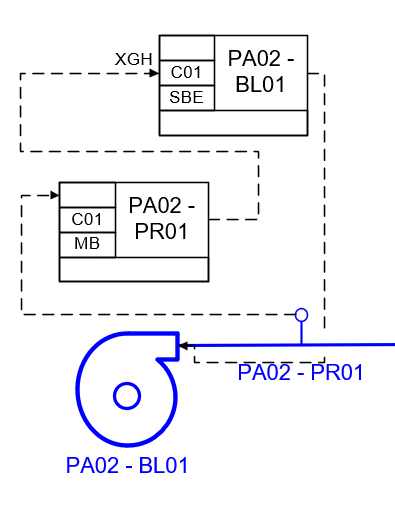
\includegraphics[width=0.8\textwidth]{Bilder/Visio_eksempel.png}
    \caption{Eksempel av \gls{SCD}}\label{fig:SCD eksempel}    
\end{figure}

\newpage